\begin{figure}
    \centering
    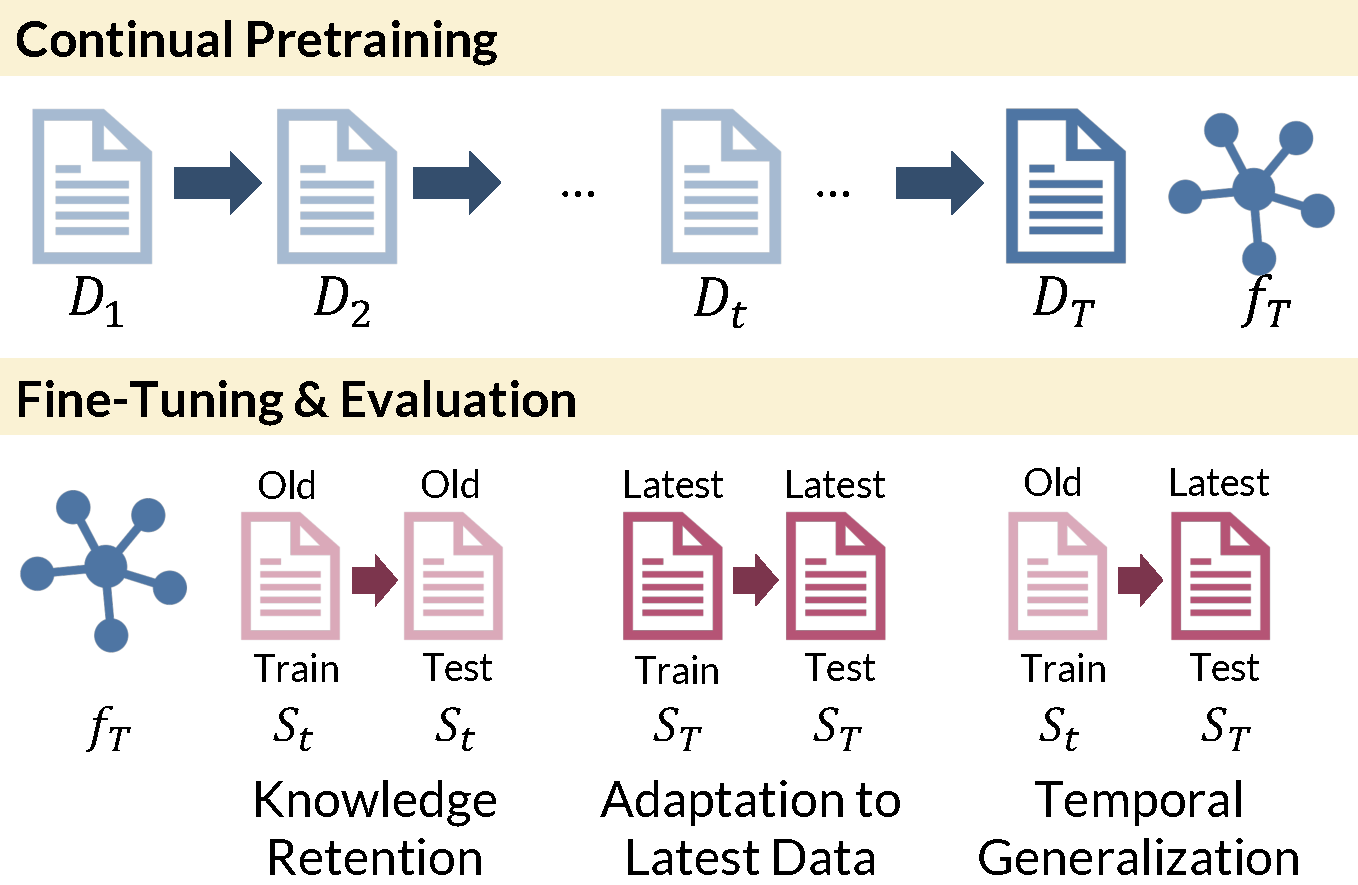
\includegraphics[width=\linewidth]{acl2022/figs/problem.pdf}
    \caption{\small \textbf{Training, evaluation setups, and metrics of lifelong language model pretraining.} The model sequentially visits each corpus, and is fine-tuned on downstream datasets related to the domains of pretraining. We evaluate knowledge retention and adaptation to new data with downstream fine-tuning performance on old and latest domains respectively. Besides, we evaluate temporal generalization where training/test examples are drawn from different time steps.
    %\xiang{need more explanation to make this figure's msgs sefl-contained. For example, I don't quite get the ``knowledge retention" and ``adaptation" part by just looking at the figure.}
   % \xiang{need to update the notations of downstream datasets.}
    }
    \label{fig:problem}
\end{figure}